\documentclass[border=1mm]{standalone}
% \usepackage[margin=2.5cm]{geometry}

\usepackage{graphicx,tikz,tikz-layers,amsmath,ifthen,tabularray} 
\usetikzlibrary{decorations.markings,calc,positioning,arrows,shapes.geometric,arrows.meta,matrix}

\colorlet{myred}{red!80!black}
\colorlet{myblue}{blue!80!black}
\colorlet{mybluee}{myblue!80!black}
\colorlet{mygreen}{green!60!black}
\colorlet{myorange}{orange!70!red!60!black}
\colorlet{mydarkred}{red!20!black}
\colorlet{mydarkblue}{blue!40!black}
\colorlet{mydarkgreen}{green!20!black}




\begin{document}

% \resizebox{\textwidth}{!}{
\tikz[font=\footnotesize, scale=1, every node/.style={outer sep=0pt, inner sep=0pt, align=center, rounded corners=0mm}, w/.style={minimum width=#1}, h/.style={minimum height=#1}, s/.style={minimum size=#1}, eu/.style={shorten >=#1}, ed/.style={shorten <=#1}, line join=round]
{
\tikzset{>={Latex[length=1.5mm, width=1.25mm]}}

\node[s=2.5cm, label={[label distance=2mm]above:Original image}] (oimage) {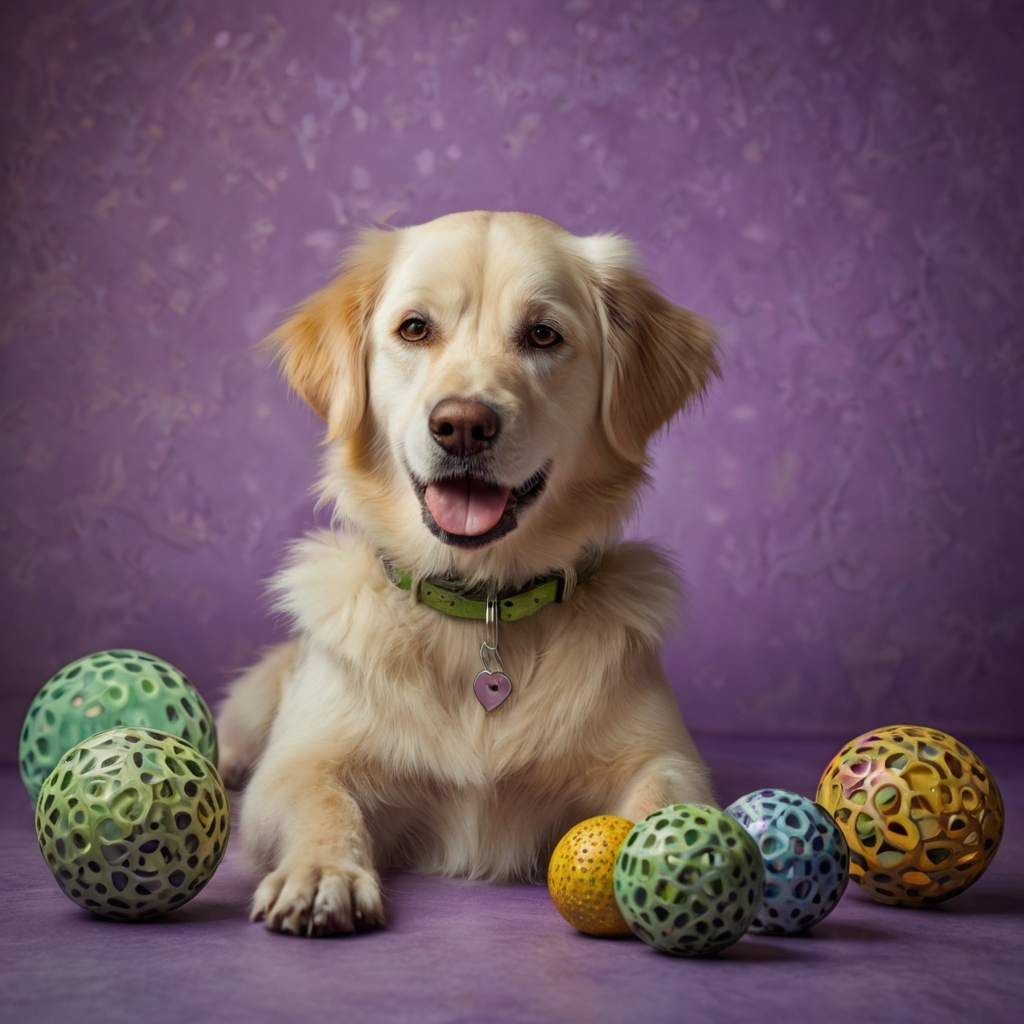
\includegraphics[width=2.5cm]{images/mosaic2/dog.jpg}};

\node[w=1.5cm, h=2.5cm, right=1cm of oimage] (tok) {Tokenizer};
\begin{scope}[on behind layer]
 \draw[fill=myblue!15] (tok.north west)--(tok.south west)--($(tok.south east)+(0,.20)$)--($(tok.north east)+(0,-.20)$)--cycle;   
\end{scope}

\node[right=1cm of tok, label={[label distance=2mm]above:Visual Tokens}] (mat) {\renewcommand{\arraystretch}{1.6}$\left[\begin{array}{rrrrr}123 & 234 & 456 & 567 \\ 987 & 876 & 765 & 543 \\ 1112 & 223 & 334 & 445 \\ 211 & 322 & 433 & 544\end{array}\right]$};

\node[w=1.5cm, h=2.5cm, right=1cm of mat, label={[label distance=2mm]above:Unused During\\Pre-Training}] (dec) {Decoder};
\begin{scope}[on behind layer]
 \draw[densely dashed, fill=myblue!15] (dec.north east)--(dec.south east)--($(dec.south west)+(0,.15)$)--($(dec.north west)+(0,-.15)$)--cycle;   
\end{scope}

\node[s=2.5cm, right=1cm of dec, label={[label distance=2mm]above:Reconstructed\\image}] (rimage) {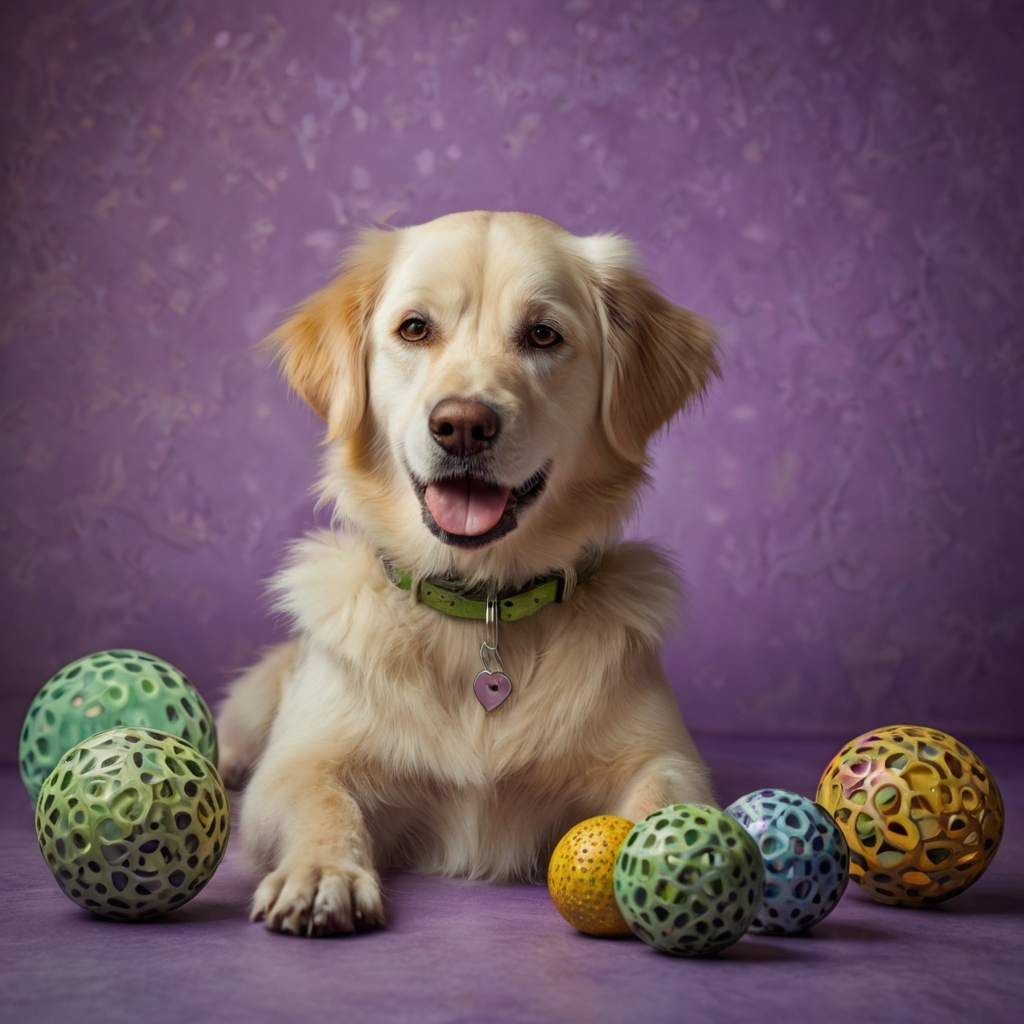
\includegraphics[width=2.5cm]{images/mosaic2/dog.jpg}};

\node[draw, densely dashed, w=5.5cm, h=3.5cm, anchor=south east] (box) at ($(rimage.south east)+(.1,-.1)$) {};

%-----------------------
\node[s=2.5cm, below=1cm of oimage, label={[label distance=1mm]above:Image Patches}] (pimage) {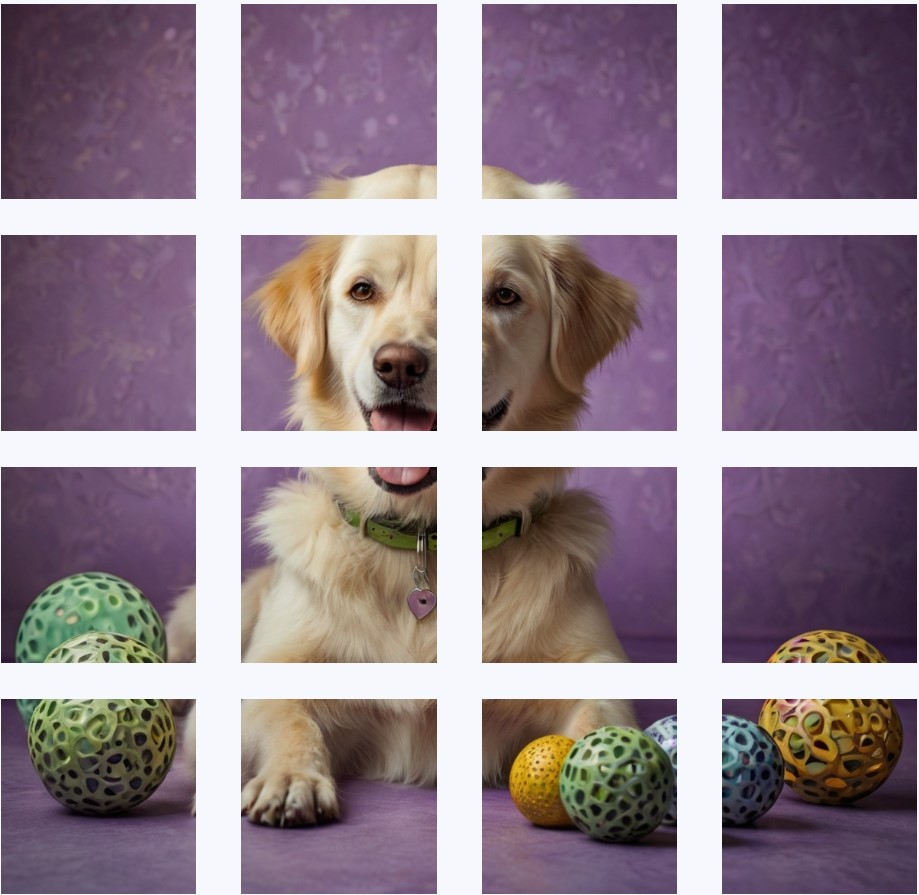
\includegraphics[width=2.5cm]{images/mosaic2/pdog.jpg}};

\node[s=2.5cm, below=1cm of pimage, label={[label distance=1mm]above:}] (eimage) {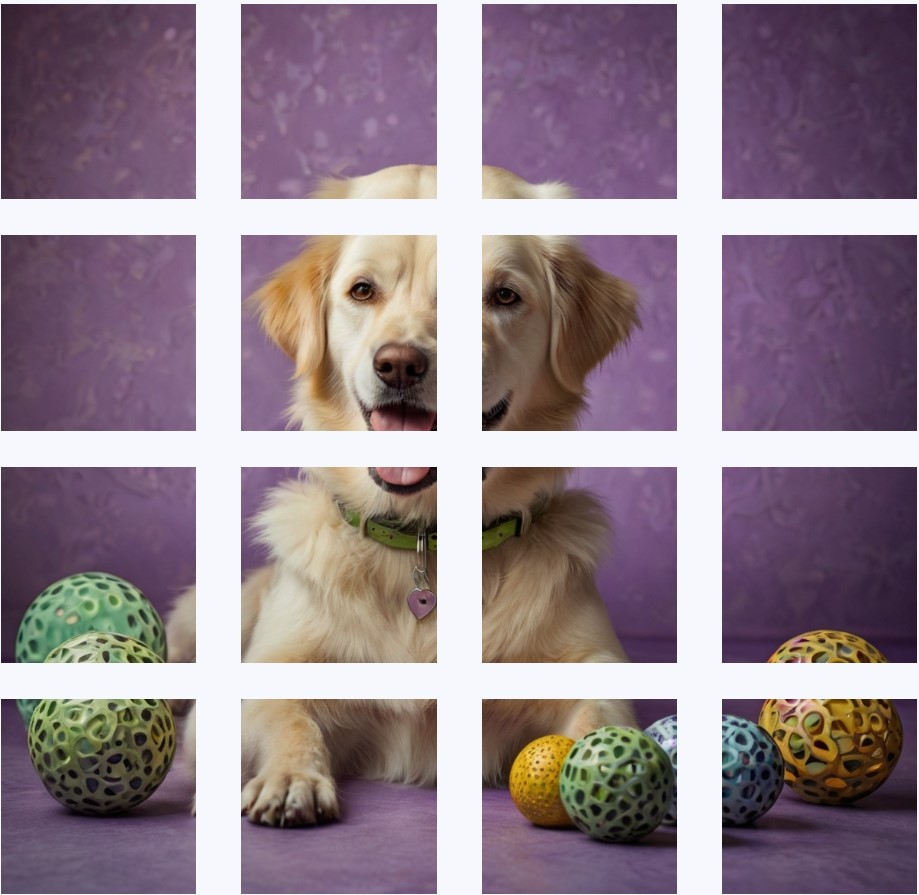
\includegraphics[width=2.5cm]{images/mosaic2/pdog.jpg}};

\node[fill=gray!50, s=.535cm, anchor=north west] at ($(eimage.north west)+(.655,-.04)$) {};
\node[fill=gray!50, s=.535cm, anchor=north west] at ($(eimage.north west)+(.655*2,-.04)$) {};
\node[fill=gray!50, s=.535cm, anchor=north west] at ($(eimage.north west)+(.655,-.67)$) {};
\node[fill=gray!50, s=.535cm, anchor=north west] at ($(eimage.north west)+(.655*2,-.67)$) {};
\node[fill=gray!50, s=.535cm, anchor=north west] at ($(eimage.north west)+(.655,-1.93)$) {};

\node[draw, w=12.35cm, h=.6cm, fill=olive!30!yellow!15, anchor=west] (mi) at (pimage-|tok.west) {Masked Image Modeling Head};

\node[draw, w=12.35cm, h=1.25cm, fill=mygreen!15, anchor=north west] (be) at ($(mi.south west)+(0,-.75)$) {\large \textbf{BEiT Encoder}};

\node[draw, s=.5cm, anchor=north west, fill=myblue!15, label={[label distance=2mm]below:$+$}] (0) at ($(be.south west)+(0,-.5)$) {0};

\foreach \i[count=\j] in {0,1,...,15}
\node[draw, s=.5cm, fill=myblue!15, right=2.4mm of \i, label={[label distance=2mm]below:$+$}] (\j)  {\j};

\node[draw, s=.5cm, below=.6cm of 0] (ss) {$[S]$};
\foreach \i in {2,3,6,7,14}
\node[s=.51cm, below=.6cm of \i, fill=gray!50] {$[M]$};


\node[below=.6cm of 1] {
\includegraphics[width=.51cm]{images/mosaic2/00.jpg}};
\node[below=.6cm of 4] {
\includegraphics[width=.51cm]{images/mosaic2/30.jpg}};
\node[below=.6cm of 5] {
\includegraphics[width=.51cm]{images/mosaic2/01.jpg}};
\node[below=.6cm of 8] {
\includegraphics[width=.51cm]{images/mosaic2/31.jpg}};
\node[below=.6cm of 9] {
\includegraphics[width=.51cm]{images/mosaic2/02.jpg}};
\node[below=.6cm of 10] {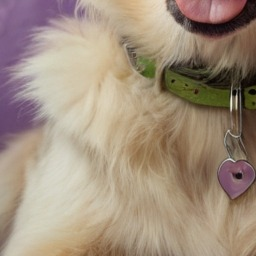
\includegraphics[width=.51cm]{images/mosaic2/12.jpg}};
\node[below=.6cm of 11] {
\includegraphics[width=.51cm]{images/mosaic2/22.jpg}};
\node[below=.6cm of 12] {
\includegraphics[width=.51cm]{images/mosaic2/32.jpg}};
\node[below=.6cm of 13] {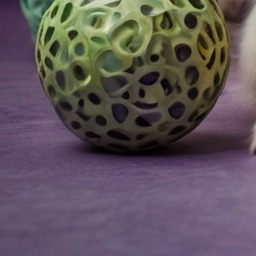
\includegraphics[width=.51cm]{images/mosaic2/03.jpg}};
\node[below=.6cm of 15] {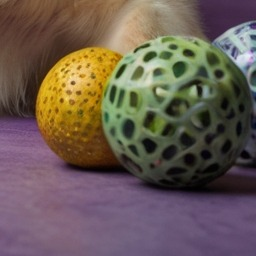
\includegraphics[width=.51cm]{images/mosaic2/23.jpg}};
\node[below=.6cm of 16] (33) {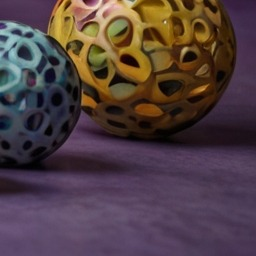
\includegraphics[width=.51cm]{images/mosaic2/33.jpg}};

\node[draw, s=.5cm, anchor=south, fill=myblue!15] (h1) at ([yshift=-1mm]be.north-|2) {\scriptsize $h^L_2$};
\node[draw, s=.5cm, anchor=south, fill=myblue!15] (h2) at ([yshift=-1mm]be.north-|3) {\scriptsize $h^L_3$};
\node[draw, s=.5cm, anchor=south, fill=myblue!15] (h6) at ([yshift=-1mm]be.north-|6) {\scriptsize $h^L_6$};
\node[draw, s=.5cm, anchor=south, fill=myblue!15] (h7) at ([yshift=-1mm]be.north-|7) {\scriptsize $h^L_7$};
\node[draw, s=.5cm, anchor=south, fill=myblue!15] (h14) at ([yshift=-1mm]be.north-|14) {\scriptsize $h^L_{14}$};

\begin{scope}[on behind layer]
\node[fill=gray!50, anchor=north, w=1.5cm, h=1cm] (sq1) at ($(mat.north)+(.06,-.06)$) {}; 
\node[fill=gray!50, anchor=south, w=.7cm, h=.4cm] (sq2) at ($(mat.south)+(-.32,.06)$) {}; 
\end{scope}

% Arrows
\draw[->] (oimage)--(tok);
\draw[->] (tok)--(mat);
\draw[->, densely dashed] (mat)--(mat-|box.west);
\draw[->, densely dashed] (dec)--(rimage);
\draw[->, eu=4mm] (oimage)--(pimage);
\draw[->] (pimage)--node[fill=white, inner sep=.5mm] {Blockwise Masking} (eimage);
\draw[->] (ss-|eimage.east)--node[below=1mm] {\tiny Flatten} (ss);

\foreach \i in {1,2,6,7,14}
\draw[->] (h\i)--(h\i|-mi.south);

\foreach \i\j in {1/234,2/456,6/876,7/765,14/322}
\draw[->] (h\i|-mi.north)--node[pos=1, above=1mm] (\j) {\j} +(0,.5);

\draw[->, densely dashed, mygreen] (sq2.south) to[out=-90,in=90, looseness=.5] (322.north);
\draw[->, densely dashed, mygreen] ($(sq1.north west)+(.3,-.4)$) to[out=-130,in=90, looseness=1] (234.north);
\draw[->, densely dashed, mygreen] ($(sq1.north west)+(.8,-1)$) to[out=-90,in=90, looseness=1] ([yshift=2mm]$(876)!.5!(765)$);

\draw[] ($(0.north west)+(0,.15)$)--coordinate[pos=.5] (w) ($(16.north east)+(0,.15)$);
\draw[->] (w)--(w|-be.south);

\node[right=2mm of 16, align=left, font=\scriptsize] {Position\\Embedding};
\node[right=2mm of 33, align=left, font=\scriptsize] {Patch\\Embedding};

}

% }



\end{document}
